% Chapter 1
\chapter{Introduction} % Main chapter title

\label{Chapter1} % For referencing the chapter elsewhere, use \ref{Chapter1} 

\lhead{Chapter 1. \emph{Introduction}} % This is for the header on each page - perhaps a shortened title

%----------------------------------------------------------------------------------------
\section{Context}
\label{context}
The rapidly progressing digital revolution have infused enormous amount of images and video, which is growing constantly. Dealing with this large scale data calls for software application for enhancing image quality, which is integral part in Image Processing. Although image processing algorithms are getting accurate day by day, there is constant pressure on algorithms to deal with noise. It is inherent to the acquisition tools. State of the art preprocessing and postprocessing algorithms are being developed to suppress noise without altering the important content. The noise in an image is reduced by convolving the image with a Gaussian function. The above common approach blurs significant features and destroys some of the geometric information in the image \citep{Thor2009}. Image processing task are often tackled with geometric methods, which targets to understand the geometric configuration and relation between the observed objects. Manifold learning algorithms are one such geometric methods.

\section{Manifold Learning}
Manifold learning is form of unsupervised machine learning algorithms, which  extract low-dimensional structure from high dimensional data. These algorithms typically try to unfold the underlying manifold so that Euclidean distance in the new space is a meaningful measure of distance metrics between any pair of points. Manifold learning assumes that the data lies approximately on a low dimensional surface embedded in a high dimensional space \citep{Tal2008}. It can be further illustrated  using figure \ref{fig:manifold}, where manifold learning algorithms for non-linear data builds an embedding function $f$ mapping $\mathcal{M}$ to $\mathbb{R}^2$.

\begin{figure}[ht]
\begin{center}
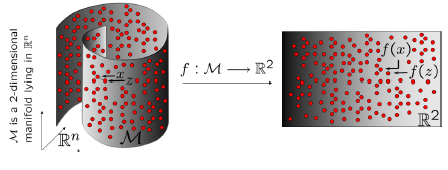
\includegraphics[width=\textwidth]{./Figures/manifold.png}
\caption{Manifold Learning \citep{Ety2008}}
\label{fig:manifold}
\end{center}
\end{figure}

\section{Motivation}

The rapidly progressing digital revolution have infused enormous amount of images and video, which is growing constantly. Dealing with this large scale data calls for algorithms, which can decipher meaningful information from the image of any quality. In any particular system, each image sequence is a point in a space of dimension equal to the number of image pixels. This in turn makes an observation space of possibly thousands/millions of dimensions. The one way to see the hope in the image data is to assume that the data is embedded as sub-manifold in high dimensional space in nonlinear way. There is no harm in assuming that that the number of free parameters remains the same throughout the observations. In line with former assumption, we also assume that there is spatially smooth variation of the parameters, then we have geometric restrictions which can be well modeled as a manifold. Learning this manifold is a natural approach to the problem of manifold learning algorithms, with the advantage of allowing nonlinear dimensionality reduction, clustering and classification.

The problem of classification of the digits is perhaps one of the most widely studied among machine learning communities. A basic requirement for credibility of classification algorithms  requires a high accuracy on MNIST datasets. Manifold learning algorithms perform under the lens of curse of dimensionality and can be best tools to classify digits. Adding to the same, the experimental results show that manifold learning algorithms can work pretty well with toy examples rather real world data. The jink associated with manifold learning has to be cleared out.


The stimulating task of anomaly detection have been studied by many researchers over the past decades. Manifold leaning algorithms too got their hands dirty to automate the anomaly detection from background pixels, but few succeed with data driven approach. We too wanted to travel in the quest of solution to the above problem using manifold learning algorithms, searching for best fit with convincing generic approach for anomaly detection.

\section{Contribution}

A through discussion of manifold learning methods require much deeper 
knowledge of manifolds, topology and differential geometry.  In this thesis, we alternatively provides intuitive ideas behind the manifold learning algorithms along with a brief description of their mathematical notions.

The research exploring the comparison of manifold learning algorithms is quite shallow. There are few theoretical comparisons results for these algorithms, but the primary evaluation methodology has been to run the
algorithm on artificial data sets and do comparison. We use MNIST datasets with optical character recognition in mind to evaluate the performance of the manifold learning algorithms.

Motivated by recent study, we presents a novel manifold learning approach for high dimensional data, with emphasis on the problem of anomaly detection in image.

\section{Organization}

The remainder of this thesis is organized as follows. Chapter \ref{Chapter2} provides mathematical background for understating the intuition behind manifold learning. After suitable mathematical background, Chapter \ref{Chapter3} provides review of intuitive ideas behind the manifold learning algorithms along with a brief description of their mathematical notions and application to image data. With necessary theory and algorithms in place, In Chapter \ref{Chapter4} we do comparison of representative manifold learning algorithms using MNIST dataset. The objective here is to accurately recognize optical character, which is in the form of handwritten digits. In Chapter \ref{Chapter5}, we presents a novel manifold learning approach for high dimensional data with emphasis on the problem of anomaly detection in image. Finally Chapter \ref{Chapter6} concludes this this thesis summary and future directions.


 

%----------------------------------------------------------------------------------------


